\section{Maschine-zu-Maschine Kommunikation}
\label{sec:MachineZuMachineKommunikation}
Bei der Maschine-zu-Maschine Kommunikation (\ac{M2M}) geht es darum, dass Maschinen automatisiert Daten miteinander austauschen können. Die Übertragungen von Daten werden dabei nicht durch Menschen ausgelöst, sondern direkt von den Maschinen. Für die Übertragung kann zum Beispiel Bluetooth, WLAN, Ethernet, Mobilfunk, ZigBee, RFID oder ein anderes Funknetzt genutzt werden. Meistens involviert ein solches Netz mehrere Geräte desselben Typs. Es werden oft auch sogenannte „M2M Area Network“ eingesetzt, damit die Geräte miteinander kommunizieren können. Diese Netzwerke haben dann meistens ein Art Router bzw. Gateway, das mit dem Internet verbunden ist.  

Das Grundkonzept ist, dass ein Gerät, bei dem es sich meistens nur um einen Mikrocontroller handelt, Daten über ein Kommunikationsnetzt an einen externen Server sendet, und dieser die Daten verarbeitet, speichert und gegebenenfalls Aktionen auslöst.

Bei M2M Kommunikation sind jedoch auch einige Hürden durch die verwendeten Geräte gegeben \cite[S. 4f]{boswarthick2012m2m}: 
\begin{itemize}
\item \textbf{Limitierte  Funktionalität} Die Geräte verfügen über wenig Rechenpower im Gegensatz zu modernen Computern. So kann ein Softwareupdate meist nicht drahtlos durchgeführt werden. Zusätzlich müssen die Geräte günstig produziert werden, was sich meistens durch an der Ausstattung bemerkbar macht. 
\item \textbf{Energiesparend } Viele Geräte die M2M nutzen sind nicht direkt an eine dauerhafte Stromversorgung angelschossen, sondern werden mit Batterien bzw. Akkus betrieben. Dies schränkt die hohe Frequenz und Datenumfang von Nachrichten ein. 
\item \textbf{Eingebettet } Die Geräte sind oft direkt in ein anderes System eingebaut, was das wechseln erschwert. Die Geräte können nur mit hohen Aufwand und einem starken Eingriff in das System ausgetauscht werden. Beispielsweise dann,  wenn die Geräte direkt in das System gelötet wurden.
\item \textbf{Langlebigkeit } Die Systeme in denen die Geräte eingesetzt werden sind oft nicht mit der normalen Lebensdauer von IT-Systemen zu vergleichen. Beispielsweise werden diese in Systemen eingesetzt die mehrere Jahrzehnte betrieben werden. 
\end{itemize}

Das Einsatzgebiet von M2M reicht von medizinischer Überwachung, Tracking von Fahrzeugen, Industrielle Anlagenüberwachung, Automatisierung von Gebäudetechnik bis zu dem Internet of Things.

\paragraph{nRF24L01 Funkmodul} Beim nRF24L01 Funkmodul handelt es sich um ein 2,4 GHz Transceiver, das für den Einsatz in Geräten mit einem sehr niedrigen Energieverbrauch ausgelegt ist. Das Funkmodul kann sowohl als Empfänger als auch Sender fungieren. Das Funkmodul kann über ein \ac{SPI} angesprochen werden. Mit Hilfe des Interfaces können auch die Register zur Konfiguration des Funkmoduls verändert werden. Das Funkmodul ist in zwei unterschiedlichen Versionen erhältlich(siehe Bild \ref{img:RF24Funkmodul}), einem Modul mit externer Antenne und einem ohne externe Antenne.

\begin{figure} [!p]
	\centering
	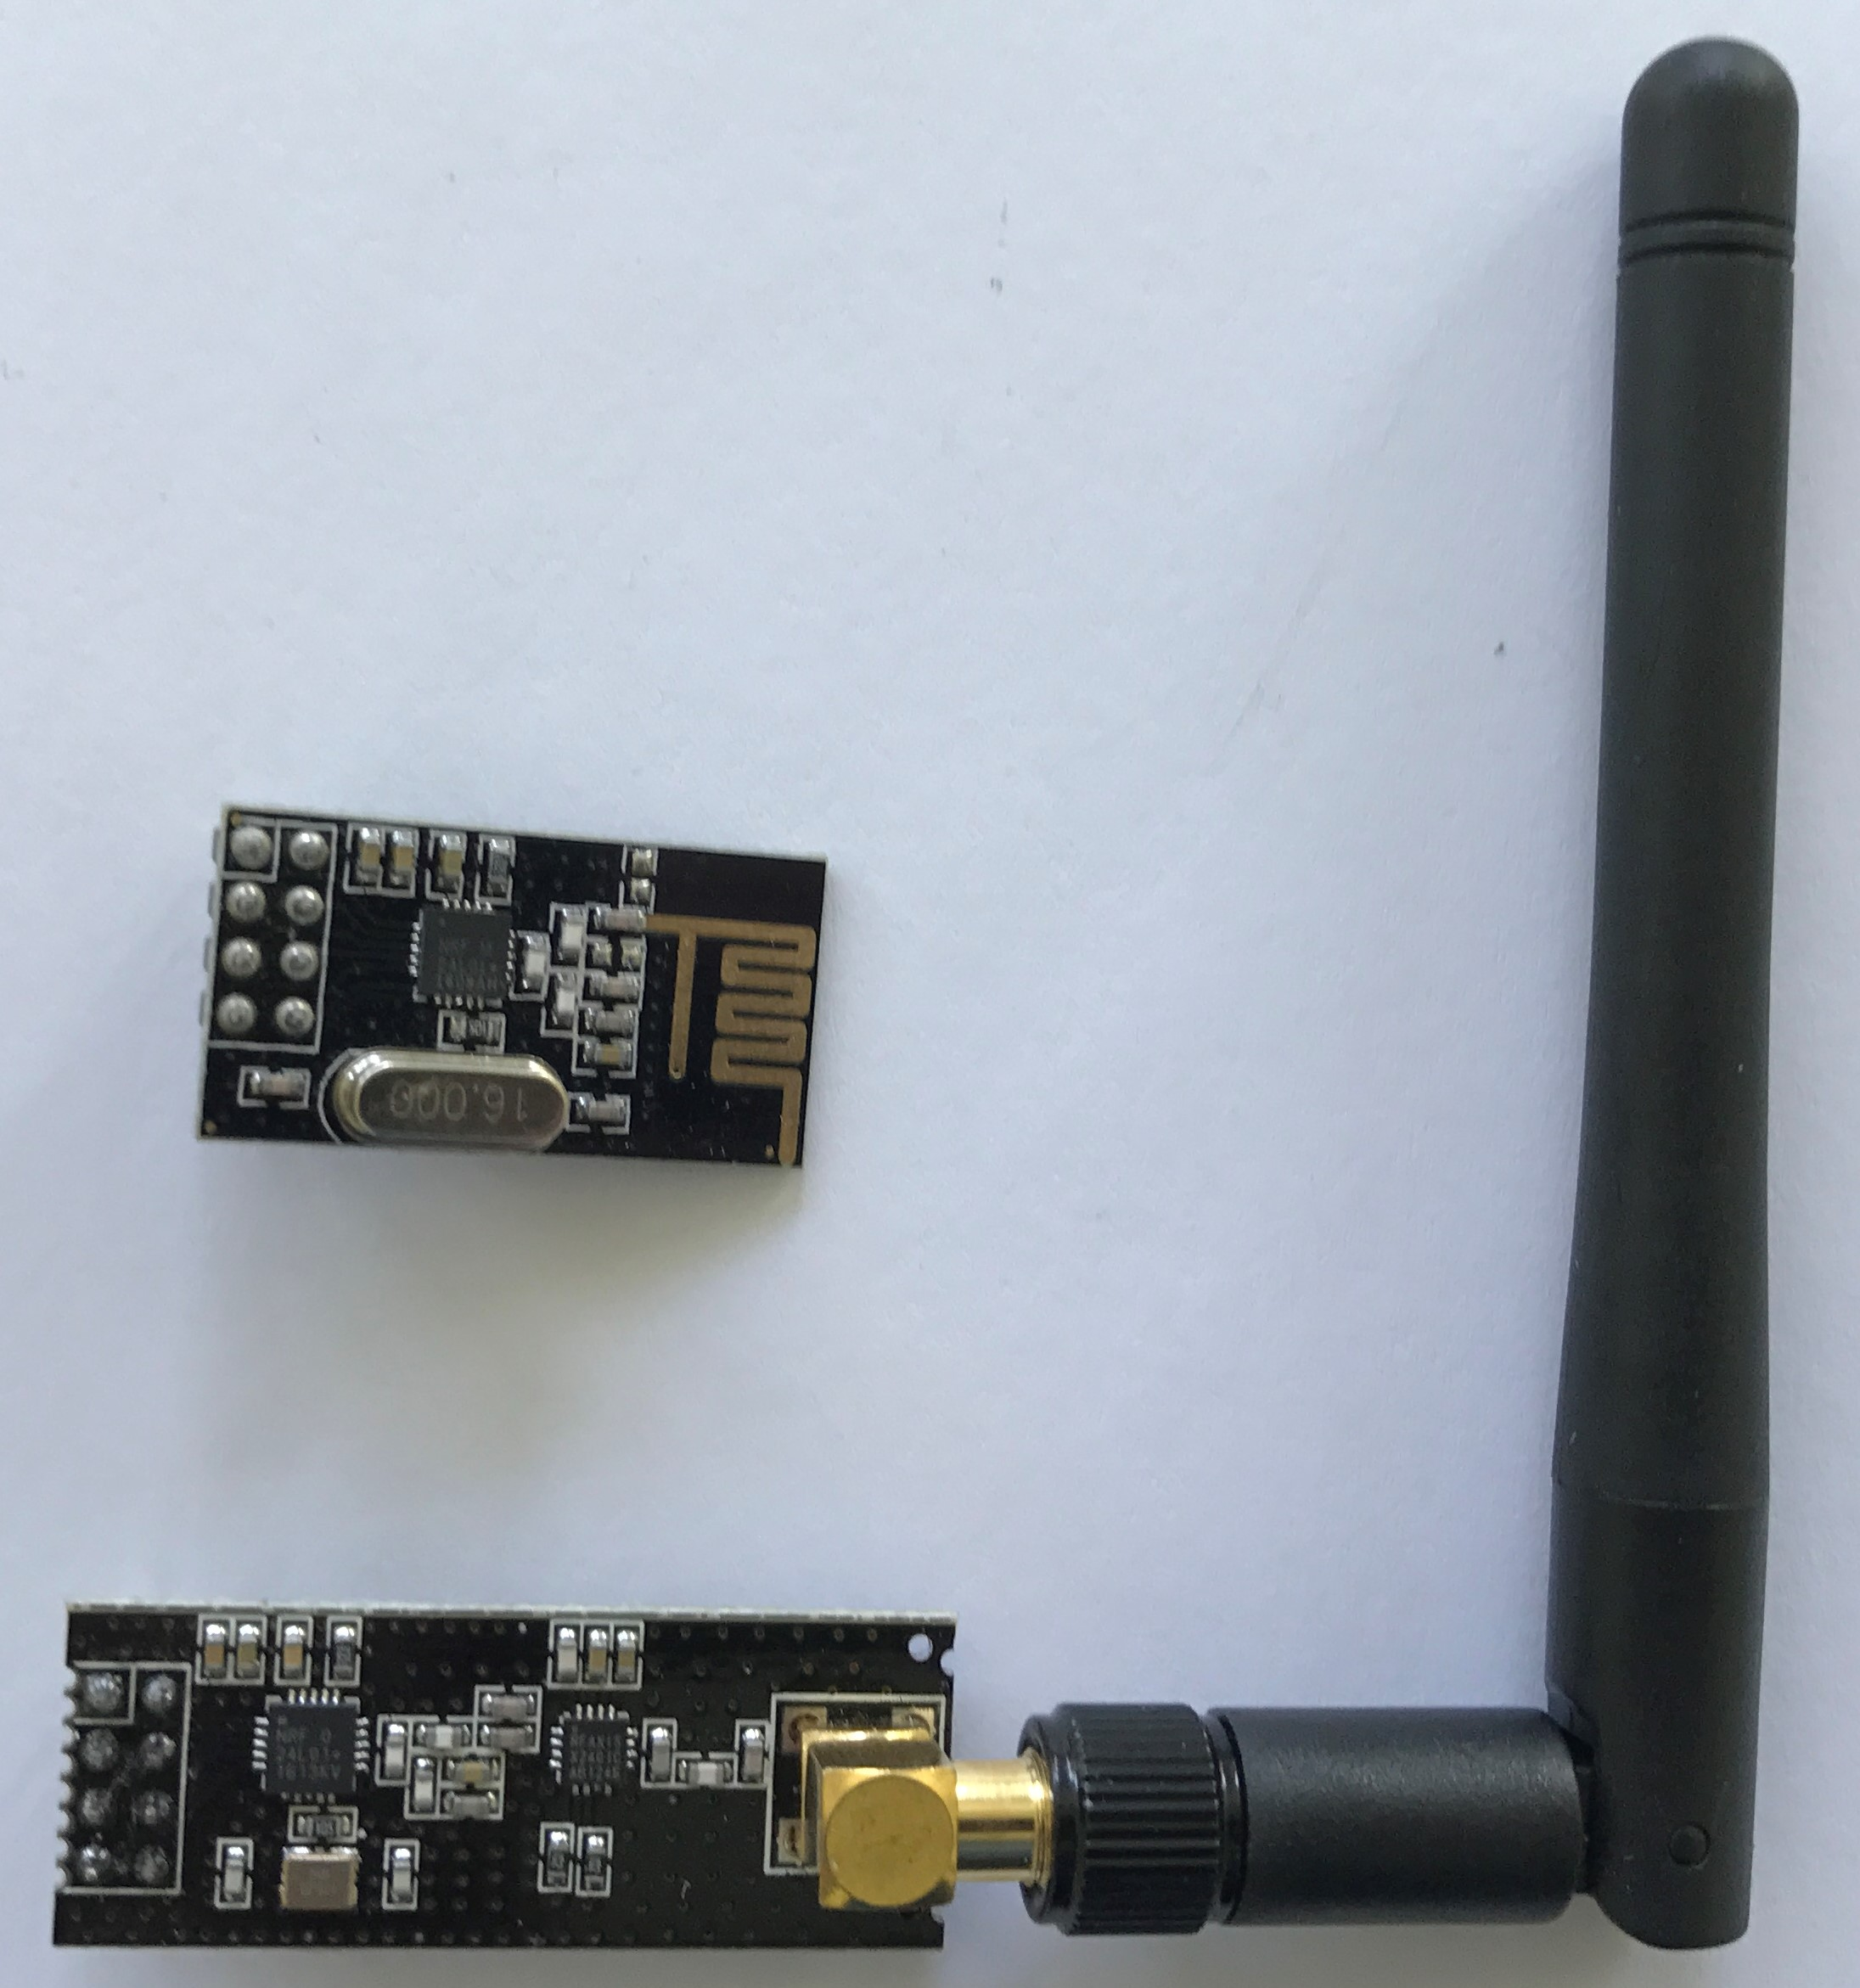
\includegraphics[width=0.45\textwidth]{bilder/RF24Funkmodul}
	\caption{nRF24L01 Funkmodule}
	\label{img:RF24Funkmodul}
\end{figure}
Zusätzlich zu den genannten Eigenschaften des Funkmoduls wird das Modul vom Hersteller Nordic Semiconducter mit folgenden Eigenschaften beworben \cite{semiconductor2007nrf24l01}:
\begin{itemize}
\item Energieverbrauch
\begin{itemize}
\item 900 nA im Power Down Modus
\item 22 $\mu$A Standby Modus
\end{itemize}
\item Datenübertragungsrate: 250 Kbps – 2 Mbps
\item Übertragungskanäle: 126
\item Betriebsspannung 1,9 – 3,6 V
\item Größe von Datenpakete: 1-32 Bytes
\item Startzeit:
\begin{itemize}
\item Power Down Modus: max. 1,5ms
\item Standby Modus: max 130 $\mu$s
\end{itemize}
\end{itemize}
